% Things to do:
%	Reframe manuscript to emphasize and interpret p-curve findings over PET-PEESE
%	See whether p-curve and PET or PEESE tend to agree
%	Bootstrapped 95 % CIs for all p-curve analyses
%	Word of warning re: trying to interpret 95 % CIs from PET-PEESE
%	Meditate on differences between additive and multiplicative error models.
%	Heterogeneity? Random effects?

% Note: Ferguson:2007a is "Evidence for publication bias"; Ferguson:2007b is "Good Bad and Ugly: Meta-analytic review"

% Bibtex is screwing up the AAP public policy statement citation. Also Konijn et al.

% It has also been widely cautioned that because trim and fill and some other techniques for assessing publication bias are based on an association between effect size and sample size, other explanations of this association should be considered. For example, effect sizes in experimental studies may be larger than those in crosssectional or longitudinal studies due to the reduced error variance that results from tight experimental controls; researchers may know this and therefore may intentionally plan to use larger sample sizes when conducting nonexperimental studies. Similarly, in some research contexts with very large sample sizes (e.g., national surveys) a researcher may have to use less precise measures (e.g., fewer items) that result in smaller effect sizes. In sum, it is possible that the effects in the studies with small samples really are larger than those in the studies with large samples (cf. Sterne and Egger, 2005). \citep[p. 152-153]{Anderson:etal:2010}
% Anderson et al also complain that \citet{Ferguson:2007a} used ``a very small set of available studies'' and ``For example, counter to widely accepted procedures for reducing the impact of publication bias, only published articles were included in the analyses and then procedures for addressing publication bias were misinterpreted. Also, studies published prior to 1995 were ignored and a large number of studies published since that time apparently were missed.'' \citep[p. 152]{Anderson:etal:2010}

\documentclass[man]{apa6}
%\documentclass{article}
\usepackage[natbibapa]{apacite}
\usepackage[longnamesfirst]{natbib}
\usepackage{pdflscape}
\usepackage{rotating}
\usepackage{csquotes}

\rightheader{Bias in Violent Games Research}
\shorttitle{Bias in Violent Games Research}

\leftheader{Hilgard et al.}

\author{Joseph Hilgard, Christopher R. Engelhardt, and Jeffrey N. Rouder}
% Broad Consensus? Open the coffin? Much ado about something out of nothing?
%\title{There Should Not Be Broad Consensus: Bias in Violent Games Research}
%Does Second Look have too much reference to Greenwald's usage in the 90s. --JR

\title{A Second Look at Bias in Violent Games Research: A Reanalysis of Anderson et al. (2010)}

\affiliation{University of Missouri}

\authornote{
Joseph Hilgard, University of Missouri-Columbia.
Please direct correspondence regarding this article to Joseph Hilgard. E-mail: jhilgard@gmail.com

THIS MANUSCRIPT HAS NOT BEEN PEER-REVIEWED. DO NOT CITE OR DISSEMINATE WITHOUT THE PERMISSION OF THE CORRESPONDING AUTHOR.}

\abstract{Violent video games are theorized to be a significant cause of aggressive thoughts, feelings, and behaviors. A meta-analysis by Anderson and colleagues (2010) is thought by some to condense the research literature into robust and incontrovertible evidence that violent video games affect these outcomes in experimental, cross-sectional, and longitudinal research. In that meta-analysis, the authors argued that there is little publication or analytic bias in the literature, applying the trim and fill procedure. However, there are now more sophisticated methods for the detection of, and adjustment for, publication bias.
In the present manuscript, we re-examine their meta-analysis and apply these new techniques for detecting bias and adjusting effect sizes. 
Our conclusions differ from those of Anderson and colleagues in three salient ways. First, we detect significant publication bias in experimental research. Second, studies selected as being ``methodologically stronger'' do not find larger effects than other studies, but instead represent a subsample of studies in which statistical significance was found. After adjusting for bias, there is no difference between the two estimates. Finally, after accounting for publication bias, effects of violent games on aggressive behavior in experimental research are found to be minimal, and effects on aggressive affect are much reduced. In contrast, the cross-sectional literature appears relatively robust and unbiased.
We outline future directions for stronger experimental research.
The results indicate the need for an open, transparent, and pre-registered research process to test the existence of the basic phenomenon.
}

\begin{document}
\maketitle


Do violent video games make their players more aggressive? Given the continued popularity of violent video games and their increasing graphical fidelity, even modest effects of violent games could have serious implications for public health. Despite decades of research and hundreds of studies, the basic phenomena remain, at least for some, controversial.  For proponents, the effects are obvious, robust, and nearly ubiquitous.  For skeptics, the research is not as clean nor the effects as obvious as has been presented.  Instead, skeptics point to a host of issues including construct validity, null findings, and publication bias as undermining the evidence for violent game effects.  In the writings of the skeptics, the evidence for the violent video game effects is not as solid as claimed; in fact, it is paper thin.

The proponents' argument is advanced by a meta-analysis from \citet{Anderson:etal:2010}.  This meta-analysis covers 381 effect-size estimates based on 130,296 participants.  These estimates were separated into ``best-practices'' and ``not-best-practices'' according to whether they met a set of inclusion criteria; the authors emphasize the best-practices subset, but provide analyses of the full sample as a sensitivity analysis. The main findings are that in best-practices experiments, there are statistically and practically significant effects of video game violence on aggressive thoughts ($r = .22$),  aggressive feelings ($r = .29$), and aggressive behaviors ($r = .21$).  Moreover, these effects not limited to experiments but are also found in cross-sectional comparisons and even in longitudinal research designs. \citet{Bushman:etal:2010} and \citet{Huesmann:2010} call the evidence in this corpus of studies ``decisive.'' 

% This paragraph is too full of hundred-dollar words and baroque turns of phrase.
Despite this meta-analysis, there are still skeptics of causal effects of violent video games on aggressive outcomes.  Skeptics are concerned that the \citet{Anderson:etal:2010} meta-analysis suffers still from purported biases in the publication of studies, the entry of effect sizes into meta-analysis, and the application of the best-practices inclusion criteria [maybe cite Ferguson, Much Ado about Nothing].  Added to this are concerns that the studies themselves suffer from questionable research practices such as the selective report of dependent variables that yield statistical significance \citep{Elson:etal:2014}. Skeptics expect that these meta-analytic biases and questionable research practices may overestimate the strength of evidence for, and magnitude of, violent video game effects.

To address this continued skepticism, we re-analyze the meta-analysis of \citet{Anderson:etal:2010}. 
First, the topic is important and controversial. Effects of violent video games are hotly debated and have implications for public health and for freedom of expression alike. Second, the \citet{Anderson:etal:2010} meta-analysis is a tremendous volume of work encompassing many studies. We were drawn to the quality and quantity of data. Finally, this is purportedly a decisive meta-analysis \citep[see][]{Huesmann:2010}. Good work deserves re-analysis; decisive work {\em requires} re-analysis.

% Organization is struggling here!
Our re-analysis provides further careful inspection of the presence or absence of the possible overestimation of violent video game effects on aggressive outcomes. First, now there are new and more effective techniques for addressing the evidentiary critiques.  These new techniques, including PET \citep[Precision-Effect Test,][]{Stanley:Doucouliagos:2014}, PEESE \citep[Precision-Effect Estimate with Standard Error,][]{Stanley:Doucouliagos:2014}, and $p$-curve \citep{Simonsohn:etal:2014,Simonsohn:etal:2014b}, provide for better adjustments for publication bias and questionable research practices than those used in \citet{Anderson:etal:2010}. 

%Second, some are concerned about the application of the inclusion criteria \citep{Elson:Ferguson:2013}. %citation missing
%Anderson et al. are admirably transparent in defining two working sets of studies---the full set of all studies and a subset of studies that meet {\em best practices} criteria.  As noted by Anderson et al., the best-practices subset yields somewhat larger effects than the full set.  For example, the violent-video-game effect on aggressive affect is $r=.29$ for the best-practices experiments but only $r=.181$ for the full set. The fact that Anderson used a best-practices set or that the effects are larger with them than the full set is not in itself of concern.  What would be of concern, however, is if study results influenced inclusion or exclusion from the best-practices set.  

\section{Concerns About Bias}
% Jeff thinks this paragraph could be more concise and more powerful.
In many ways, it would be remarkable if violent video game effects were not at least somewhat overestimated, as biases that overestimate effect sizes are extremely common in science.
In recent years, psychology has experienced a crisis of confidence as researchers realize that many published research findings may not replicate. In an attempt to replicate the results of 100 psychology studies, only 39 studies yielded the same significant effect \citep{OpenScienceCollaboration:2015}. Critics have pointed out that hypothesis-confirming results appear in the literature much more frequently than would be expected given reasonable estimates of statistical power \citep[see][]{Schimmack:2012}. Statistical oddities are not limited to unusually significant results, however. Using statistical techniques and reporting standards typical of social psychology, researchers have been able to provide experimental evidence for impossible phenomena such as extra-sensory precogition \citep{Bem:2011} and a song that makes its listeners younger \citep{Simmons:etal:2011}. 
It has even been suggested that the current ``publish or perish'' reward structure of academia encourages researchers to publish as many Type I errors as possible, which researchers can accomplish by conducting many small, weak studies and using biased analytic techniques \citep{Bakker:etal:2012}. In this light, one might expect that there could be bias in violent games research, as there is in so many other literatures. 

We were concerned about three potential sources of bias in the Anderson et al. meta-analysis. The first, {\em publication bias}, is the phenomenon that studies with statistically significant (i.e., $p<.05$) findings are more likely to be submitted and accepted for publication. The second, $p$-hacking, is the possibility that researchers increase their Type I error rates in an attempt to find publishable, statistically significant results. The last, {\em selection bias}, is the application of flexibility in meta-analytic inclusion criteria. We discuss each in turn.

\subsubsection{Publication bias}
Publication bias is a problem that contributes to the overestimation of effect sizes and the propagation of Type I error. It is an especially dangerous problem for meta-analysis, as the selective reporting of studies that attain significance leads to an overestimated effect size and may lead to unwarranted conclusions of statistically and practically significant effects. The error introduced by publication bias is larger when research studies are comprised of smaller samples and are consequently underpowered.  For these small-sample studies, only those that overestimate the effect dramatically are able to reach the threshold of statistical significance. Hence, small studies with large effects are perhaps the most suspect.  

The critical question is whether there is evidence for publication bias in the violent video-game literature as synthesized by \citet{Anderson:etal:2010}.  Here there is disagreement.  Anderson et al. claim that there is little evidence for publication bias.  Their claim follows from their attempt to account for such bias.  They used a  trim-and-fill procedure, which we discuss subsequently, to estimate bias-adjusted effect size estimates. This procedure recommended only a small adjustment, thereby suggesting a minimal degree of publication bias. This claim has two weaknesses.  First, the trim-and-fill correction is understood to be not particularly effective, as it corrects for bias when bias is absent and does not correct enough when bias is strong \citep{Simonsohn:etal:2014b}. \citet{Ferguson:2007}, in contrast, makes the case that publication bias is a problem in the violent-video-game literature through application of Egger's regression test. Second, the authors found 16 dissertations which had yielded nonsigificant results and subsequently gone unpublished, but only one unpublished non-dissertation study. Given that dissertations likely represent a minority of all studies conducted on violent games, one might expect that there are more unpublished studies yet languishing in file drawers. In our view, the claim that there is minimal publication bias in violent media seems implausible given the prevalence of publication bias in research in general and in social psychology in particular.  On this basis, more detailed consideration of the possibility of bias in the Anderson et al. meta-analytic dataset is warranted.

\subsubsection{$p$-hacking}
Because statistically significant results are easier to publish, particularly in prestigious journals, researchers often strive for statistical significance. Often, this striving leads to the desired statistical significance but also causes an inflated Type I error rate; the obtained result is more likely to be a false positive. Some such practices include data-dependent stopping (i.e., deciding to end data collection when $p < .05$ or continue when $p > .05$), the strategic inclusion or exclusion of outliers depending on their influence on the results, or the analysis of subgroups when results for the whole sample are not found.

We suspect there are two specific $p$-hacking mechanisms in the violent-video game literature.  The first involves the strategic use of dependent measures.  In this literature, it is common to collect several dependent measures.  For example, some researchers measure aggressive behavior by allowing participants to administer a painful burst of noise to another participant. Both the volume and duration of such a noise burst are measured.  There is considerable diversity in the way studies have combined these quantities, and it has been suggested that the diversity reflects the fact that some studies find statistical significance under one combination while other studies find significance under a different combination \citep{Elson:etal:2014}.  In general, when researchers collect several dependent measures, there exists the possibility that there is some strategic selection among them.  

% need to elaborate on this next section -- strategic inclusion of covariates is one form of p-hacking and I don't have evidence for or against it. However, I do think an amount of subgroup analysis goes on vis-a-vis p-hacking.
A second mechanism is the strategic analysis and presentation of subgroups. For example, in \citet{Anderson:etal:2004}, study 2, participants played a violent or nonviolent game and were then either clearly or ambiguously provoked by a confederate. In their meta-analysis, Anderson et al. include only those participants in the ambiguous-provocation condition. This selective inclusion was applied in both the best-practices and full-sample analyses. In personal correspondence, Anderson tells us, ``Only the ambiguous provocation condition was used because we now know that the unambiguous (increasing) provocation version of the task is not as sensitive to a variety of independent variables as is the ambiguous provocation pattern.'' (Personal communication, Nov. 4, 2014). 
We find this approach risks capitalizing on chance, allowing extra opportunities for an effect to be detected and thereby increasing familywise error rates.

\subsubsection{Selection bias}
Selection bias may contaminate meta-analysis when the researchers include or exclude studies on the basis of the hypothesis they favor. The application of the best-practices inclusion criteria applied by Anderson et al. was the subject of some controversy. Skeptics argued that the inclusion criteria were applied more liberally to studies with significant results than to studies with nonsignificant results. [cite Ferguson, 2010? Elson \& Ferguson, 2013?] If this is the case, then the best-practices subset may find larger effects not due to stronger methodology, but because of greater overestimation through selection bias. 

\section{Assessing Bias in Meta-Analysis}
There are several approaches to assessing the aforementioned biases in meta-analysis, and some of these have been developed since the publication of \citet{Anderson:etal:2010}. We used several of the more recent tests and methods to provide a new perspective on the Anderson et al. meta-analysis.

A common theme of many of these methods is the relationship between effect size and precision (or sample size) in reported studies. Because sample size does not typically cause effect size, an unbiased research literature is expected to have no relationship between effect size and precision. However, such a relationship will be observed if studies must attain statistical significance to be published. Small-sample studies require large observed effect sizes to reach statistical significance, while large-sample studies can reach statistical significance with smaller observed effect sizes. Thus, in the presence of publication bias, there is an inverse relationship between effect size and precision. 

Note that, in some cases, sample size and effect size may be correlated for reasons other than bias. For example, experimental studies tend to have smaller samples than correlational studies, and each paradigm may reflect different underlying effect sizes. Alternatively, it may be possible that manipulations and measurements in small samples are more effective than in large samples. To represent these possibilities, a relationship between sample size and effect size is often called ``small-study effects'' rather than ``publication bias.'' Some of these possibilities can be excluded through practice; conducting separate bias tests for correlational and experimental research can rule out study design as a potential cause of small-study effects.

\subsubsection{Funnel plots}
A funnel plot summarizes the relationship between effect size and sample size, allowing for visual estimation of small-study effects. In a funnel plot, effect size is plotted on the x-axis and precision on the y-axis. In the absence of small-study effects or heterogeneity, study results will form a symmetrical funnel shape, displaying substantial variance when sampling error is large but narrowing to a precise estimate when sampling error is small. Because of this sampling error, some small-sample studies are expected to find null or even negative results even when the underlying effect is positive, so long as there is not bias. The funnel should fill symmetrically. See Figure~\ref{funnels1}A for an example of a funnel plot of a simulated unbiased research literature.

Such symmetry is not found in funnel plots of research contaminated with publication bias or $p$-hacking.  In the case of publication bias, studies are missing from the lower portion of the funnel where results would not reach statistical significance. See Figure~\ref{funnels1}B for such an asymmetrical funnel plot, generated by simulating a biased research literature. Funnel-plot asymmetry can also be caused by flexibility in analysis and report. When samples are collected until a desired $p$-value is attained, published studies will increase in both precision and effect size, moving towards the upper-right edge of the funnel. When subgroups or experimental subgroups are dropped from report to highlight only a subgroup in which statistical significance was found, studies will lose precision and increase in effect size, moving towards the lower-right edge of the funnel. When outcomes are censored from report to highlight only the significant outcomes, the effect size increases, moving studies to the right of the funnel.   %JOE, WE NEED A FIGURE, AND I AM NOT SURE I BUY THIS.  CAN YOU RUN A SIM.  % Maybe I'll make a figure. I am not programming a bunch of simulations. We can talk about it if you need to.

Although funnel plots provide a useful graphical representation of bias, they are, unfortunately, omitted in \citet{Anderson:etal:2010}.  This makes it difficult for readers to appraise the strength of the data, inspect the distribution of study results, identify possible mis-entered values, and determine whether the na{\"i}ve (that is, unadjusted) and trim-and-fill effect size estimates might be influenced by outliers. We provide them in this report. 

% Trim-and-fill and how it's bad
\subsubsection{Trim and fill}
One popular bias-adjustment technique, trim-and-fill \citep{Duval:Tweedie:2000}, attempts to detect and adjust for bias through inspection of the number of studies with extreme effect size estimates on either side of the meta-analytic mean estimate. If the funnel plot is asymmetrical, the procedure ``trims'' off the most extreme study and imputes a hypothetical censored study reflected around the funnel plot's axis of symmetry (e.g., an imputed study with a much smaller or even negative effect size estimate). Studies are trimmed and filled in this manner until the ranks are roughly equal. See Figures~\ref{funnels1}C and ~\ref{funnels1}D for examples of trim-and-fill adjusted funnel plots of simulated biased and unbiased literatures, respectively. 

However intuitive, this is not an especially effective adjustment for bias, as the assumptions of trim-and-fill are unlikely to be met \citep{Simonsohn:etal:2014b}. Studies are not likely to be censored on the basis of the effect size, but rather, on the basis of their statistical significance. Accordingly, it is argued that trim-and-fill does a poor job of providing an adjusted effect size, adjusting too much when there is no bias and adjusting too little when there is bias \citep{Simonsohn:etal:2014b}. %Could cite other sources via Lakens blog post
(Indeed, our simulated datasets in Figures~\ref{funnels1}C and ~\ref{funnels1}D experience both these problems; however, they are single simulation runs and may not represent the long-run behavior of trim-and-fill.) %These are the data colada blog post and lakens' comment blog post
%(c.f. Duvall \& Tweedie, 2000, who argue that suppression via $p$-value is too simplistic and that there is little difference between the two)
% I had Peters, 2007 as a potential citation elsewhere in the paper, too. And I could look at Moreno et al. to see how trim-and-fill performed relative to metaregression.
The imputation of additional effect sizes also must be regarded with caution, as it adds information to the dataset that does not necessarily exist (Higgins \& Green, 2011). 
\nocite{Higgins:Green:2011}
%%Cochrane Handbook for Systematic Reviews of Interventions, March 2011, v5.1.0) %url: http://handbook.cochrane.org/chapter_10/10_4_4_2_trim_and_fill.htm

For these reasons, trim-and-fill is most commonly suggested as a form of sensitivity analysis rather than a serious estimate of the unbiased effect size. When the na{\"i}ve meta-analytic estimate and the trim-and-fill-adjusted estimate differ only slightly, it is suggested that the research is largely unbiased; when the difference is large, it suggests potential research bias.
\citet{Anderson:etal:2010} applied trim and fill in their meta-analysis as the only attempt to detect and adjust for small-study effects. Trim-and-fill yielded only slightly-adjusted effect sizes, and so the authors concluded minimal research bias.  %Although we are confused by their decision to divide by culture and not to perform trim-and-fill on the total sample -- the smaller the sample, the poorer the power to detect asymmetry, perhaps?
%Some have characterized this as an extensive test for publication bias \citep[][pg. 51]{Bushman:Huesmann:2014} despite the weaknesses of the trim-and-fill procedure and the absence of funnel plots or other tests for bias.
In our opinion, a conclusive test for bias requires more thorough testing than trim-and-fill alone can provide \citep[c.f.,][]{Bushman:Huesmann:2014}.

\subsubsection{Egger's regression test}
Egger's regression test \citep{Egger:1997} is a simple check for bias which inspects the degree and statistical significance of the relationship between sample size and effect size. A significant test statistic suggests that the observed funnel plot would be unusually asymmetrical if the collected literature were unbiased. This test is sometimes helpful in reducing the subjectivity in visually inspecting a funnel plot for asymmetry. Figures~\ref{funnels1}E and ~\ref{funnels1}F show unbiased and biased simulated research literatures with overlaid Egger regression lines. The unbiased literature does not have a significant slope, but the biased literature does. 

One weakness of Egger's regression test is that, while it can detect bias, it does not provide a bias-adjusted effect size. The test is also known to have poor statistical power when bias is moderate or studies are few, limiting the strength of conclusions that can be drawn through application of the test (Sterne, Gavaghan, and Egger, 2000).

Egger's regression test has been used repeatedly by skeptics to look for publication bias \citep[e.g.,][]{Ferguson:2007,Ferguson:Kilburn:2009}, but was not reported in the \citet{Anderson:etal:2010} meta-analysis. Although Anderson and colleagues argue that their analysis contains minimal publication bias, an Egger's regression test might have found significant bias.

\subsubsection{PET-PEESE meta-regression}
A promising new tool in the detection of and adjustment for bias is meta-regression. Meta-regression estimates a bias-adjusted effect size by considering the relationship between effect size and precision, then estimating the underlying effect size that would be found with perfect precision. Two meta-regression estimators are the Precision-Effect Test (PET) and Precision-Effect Estimate with Standard Error (PEESE) \citep{Stanley:Doucouliagos:2014}. %See carter & McCullough for better citations 

In PET, a weighted {\em linear} regression is fit to describe the relationship between effect size and precision, much like the Egger regression test. Unlike Egger's test, however, PET then extrapolates from this regression to estimate what the effect would be in a hypothetical study with perfect precision. When there is minimal bias, there is minimal adjustment (see the simulation in Figure~\ref{funnels2}A). When there is no underlying effect, published studies tend to lie on the boundary between statistical significance and nonsignificance, forming a linear relationship between sample size and precision. Thus, PET performs well at estimating effects when the underlying effect is approximately zero (see the simulation in Figure~\ref{funnels2}C). PET performs less well when there is some effect. When there is an underlying effect, small studies will be censored by publication bias, but most large studies will find statistical significance and be unaffected by bias. PET will fail to model this nuance and risks underestimating the size of nonzero effects (see the simulation in Figure~\ref{funnels2}B).

A second meta-regression estimator, PEESE, is intended to address this problem. PEESE fits a weighted {\em quadratic} relationship between effect size and precision. The resulting curve models bias as being stronger in the lower part of the funnel but reduced as the studies become better-powered and less subject to censoring. Again, in the absence of bias, adjustment is minimal (see the simulation in Figure~\ref{funnels2}D). PEESE is less likely than PET to underestimate nonzero effects (Figure~\ref{funnels2}E), but risks overestimating the size of null effects (Figure~\ref{funnels2}F).

Because PET underestimates nonzero effects and PEESE overestimates null effects, sometimes PET and PEESE are combined as a two-step conditional PET-PEESE procedure. If PET detects a significant effect, the PEESE estimate is used; if PET does not detect a significant effect, the PET estimate is used. Although this approach would seem to make use of the estimators' complementary strengths and weaknesses, this approach may be exceedingly conservative, as PET has questionable statistical power for the detection of effects. When PET's power is poor, conditional PET-PEESE tends to underestimate effects, as only PET is ever applied. For this reason, we report both PET and PEESE. When the PET estimate is significant, the PEESE estimate should be favored, but when it is not significant, we do not necessarily favor PET over PEESE, as non-significant results do not guarantee the truth of the null hypothesis.

These meta-regression techniques have been previously applied by \citet{Carter:McCullough:2014} to inspect the amount of evidence for ``ego depletion,'' the phenomenon of fatigue in self-control. They found that after adjusting for small-study effects, PET-PEESE suggested an absence of evidence for the phenomenon. The authors therefore recommended a large-sample pre-registered replication effort, now supported by the American Psychological Society as the topic of the third Registered Replication Report (http://www.psychologicalscience.org/index.php/publications/observer/obsonline/aps-announces-third-replication-project.html).

% Explaining that I'm basically using Peters
% Maybe this would be a good one for 
One criticism of the Egger and PET-PEESE metaregression tests is that some effect size estimates have an inherent relationship between precision and effect size that is not caused by research bias. For example, given a single sample size, the precision of Cohen's $d$ increases as the effect size $d$ increases. A similar phenomenon holds for odds ratio. When these effect sizes are used, metaregression techniques risk misidentifying the inherent relationship between precision and effect size as a small-study effect. To avoid this problem, it has been suggested that one instead use precision estimates that are a function of the sample size alone (Peters, Sutton, Jones, Abrams, \& Rushton, 2006). In the current report, we use as our effect size estimate Fisher's Z with standard error $\frac{1}{\sqrt{N-3}}$, consistent with the original analysis of Anderson and colleagues. Because this standard error is not a function of the effect size, we avoid the problem of an inherent relationship between precision and effect size that might otherwise contaminate the metaregression.

\subsubsection{$p$-Curve}
Another novel technique for accounting for small-study effects is $p$-curve \citep{Simonsohn:etal:2014,Simonsohn:etal:2014b}. $p$-curve estimates the underlying effect size by inspecting the distribution of significant $p$-values. 
% How do I talk about this without resort to true/false terms?
When the null hypothesis is true (i.e. $\delta$ = 0), the $p$-curve is flat: significant $p$-values are as likely to be between .00 and .01 as they are between .04 and .05. When the null hypothesis is false, the $p$-curve becomes right-skewed such that $p$-values between .00 and .01 are more common than are $p$-values between .04 and .05. The degree of right skew is proportionate to the power of studies to detect an effect such that increasing sample sizes or larger true effect sizes will yield greater degrees of right skew. By considering the $p$-values and sample sizes of significant studies, $p$-curve can be used to generate a maximum-likelihood estimate of the true effect size.

One weakness of $p$-curve is that, in the presence of questionable research practices, an excess of $p$-values will gather just under the $p$ = .05 threshold. This results in a flatter $p$-curve than would be found if studies had been reported without $p$-hacking, and thus $p$-curve will underestimate the true effect size in these circumstances. That aside, simulation work suggests that $p$-curve is quite effective at estimating true effect sizes \citep{Simonsohn:etal:2014,Simonsohn:etal:2014b}.

In summary, we will apply a number of meta-analytic techniques for detecting and adjusting for publication bias. Funnel plots provide a graphical presentation of possible biases, while the Egger test provides a formal statistical test for bias. $P$-curve, PET, and PEESE provide adjusted effect size estimates.

\subsection{Unpublished Materials}
Publication bias, in which journals tend to publish only significant findings, is a chief source of overestimated effect sizes in meta-analysis. Nonsignificant results can be difficult to retrieve for meta-analysis as they often go unpublished and forgotten. However, one publication format is largely immune to these publication pressures: the doctoral dissertation. Department requirements generally dictate that dissertations be submitted and published in a dissertation database regardless of whether or not that dissertation is later published as a peer-reviewed journal article.  Another advantage of dissertations is that they are typically thorough, reporting all outcomes and manipulations, whereas published journal articles may instead highlight only the significant results.  Dissertations, then, provide us with a sample of reported studies relatively uncontaminated by publication biases favoring significant results. In our analyses, we examine unpublished dissertations, their patterns of statistical significance, and how they fared in meeting best-practices criteria.

\section{Method}
We perform a reanalysis of the \citet{Anderson:etal:2010} meta-analysis using the data as provided by the study's first author.  We augment the trim-and-fill approach with funnel plots, PET and PEESE meta-regression, and $p$-curve effect-size estimation. We use the original authors' separation of studies by study design (experimental, cross-sectional, longitudinal) and by study outcome (affect, behavior, cognition, arousal) in our presentation.

\subsection{Aggregation of rows}
We assume that entire studies are censored or re-analyzed per their statistical significance. However, the original data have some studies split across multiple rows in order to test for moderators. For example, one study might have two rows: one for the simple effect among males, and another for the simple effect among females. Where multiple effects were entered for a single study, we aggregated these to form a single row by summing the sample sizes and making a weighted average of the subsample effect sizes. This parallels the behavior of the software used in the original analysis. 

\subsection{Calculation of $p$-values}
Although the original data entry performed by Anderson and colleagues is admirably thorough, the data set given us does not have the necessary statistics for $p$-curve meta-analysis. We calculated $t$-values by dividing Fisher's Z scores by their standard errors, then used the $t$-value to calculate a two-tailed $p$-value. We do not report a $p$-value disclosure table as recommended by \citet{Simonsohn:etal:2014}, as the meta-analyzed $p$-values are a function of the data as entered by Anderson et al. and not a direct entry of $p$-values from manuscripts.
%We consulted with the original authors as how best to aggregate rows within studies and reproduce their provided estimates. % Anderson has lost patience with me, I doubt we will be consulting anytime soon.
%Trying to explain this per Randy McCarthy suggestion
Although $p$-curve is most often applied to look for evidence or bias in primary study hypotheses, it can also be used to aggregate main effects across studies by examination of the associated $p$-values.

\subsection{Adjusted estimates}
PET and PEESE meta-analytic adjustments were calculated. PET was performed by fitting a weighted-least-squares regression model predicting effect size as a linear function of the standard error with weights inversely proportional to the square of the standard error. PEESE was also performed, predicting effect size as a quadratic function of the standard error and using similar weights. Finally, $p$-curve effect size estimates were generated using code provided by \citet{Simonsohn:etal:2014}, entering a $t$-value and degrees of freedom parameter for each relevant study.

Within the meta-regressions, all effect sizes were converted to Fischer's Z so as to fulfill the meta-regression model's assumptions of normally-distributed errors. All meta-regressions were performed using the `metafor' package for {\bf R} (Viechtbauer, 2010), using the {\tt rma()} function to fit a weighted model with an additive error term. Effect sizes are converted back to Pearson $r$ for tables and discussion. 
$p$-curve estimates were similarly converted from Cohen's $d$ to Pearson $r$ for consistency of presentation.
\nocite{Viechtbauer:2010} % same for Egger test? It's just the slope from PET, right?

PET, PEESE, and $p$-curve are likely to perform poorly when there are few datapoints. Therefore, our analysis is restricted to effects and experimental paradigms with at least ten independent effect sizes. %citation needed from Carter & McCullough, 2014
Our code has been made available online at https://collaborate.missouri.edu/jhilgard/craig\_meta in the case that the reader nevertheless wants to generate estimates for more sparse datasets or explore the impact of our inclusion and exclusion decisions. The data are available upon request from Dr. Anderson. % Need Craig's permission. % Need to clone to public resource GitHub

\subsubsection{Sensitivity analysis}
In addition to our analysis of the full dataset as provided by Anderson and colleagues, we perform leave-one-out sensitivity analyses, removing each datapoint one at a time and making all adjusted estimates. For each analysis, a supplementary tab-delimited spreadsheet is attached that lists the individual studies and the estimates when they are left out.\footnote{Initially, we had attempted a different sensitivity analysis in which we removed datapoints with a Cook's distance of more than 0.5 on the PET regression. In the case that several observations were excessively influential, we performed an iterative procedure, deleting the single most influential observation and checking again for influence until no observations had excessive influence. In practice, this tended to delete all datapoints that did not fit the PET regression well. This seemed to distastefully and unfairly favor the PET model over the available data, so we eschewed this approach.} %consider summarizing in text?

\subsection{Studies excluded}
We removed three studies from meta-analysis due to concerns over relevance and accuracy. First, \citet[study 1]{Matsuzaki:etal:2004} was removed because its entered effect sizes were unusually large for their precision (i.e., effects on aggressive behavior $r = .60$ and aggressive cognition $r = .53$), were highly influential on the meta-regression model, and could not be found as entered in the \citet{Anderson:etal:2010} dataset by inspection of the original article.%\footnote{We asked Dr. Anderson for comment. He replied, ``The Japanese team reported additional results for a number of their papers, in those cases in which the initial paper didn't have what was needed. This was true for several other papers as well. For example, if an original paper reported only some composite measure of aggressive personality but had more specific data on physical aggressiveness, we tried to get the more appropriate measure.'' It seems unlikely to us that such a large effect would be found on a single most-appropriate measure and nevertheless would go unreported in favor of a smaller composite effect. However, it is certainly possible. Without recourse to the raw data, we omit this study as an outlier and probable error of data entry.}
\citet{Panee:Ballard:2002} was removed because the study tested the effects of violent primes on in-game behaviors, not the effects of violent gameplay on aggressive outcomes; therefore, it does not provide a relevant test of the hypothesis. 
Finally, \citet{Graybill:etal:1985} was removed from analysis. As entered in the Anderson et al. dataset, the effect size was unusually large and significant, $r = 0.57, p = 1.6 \times 10^{-10}$. The cause of this enormous outcome was that the study's manipulation checks were entered as though they were primary study outcomes on aggressive cognitions. %Participants were asked ``Tell me what happened in the video game you played,'' and ``What did you like about the video game you played?'' The results of the chi-square tests on these manipulation checks were then averaged together with two non-significant psycho-analytic outcomes. %While what is meant by ``aggressive cognition'' is not exactly clear, we do not think this manipulation check provides a relevant test.

% Anderson et al. It would be nice to provide trim-and-fill estimates, maybe?
\subsection{Subsets re-analyzed}
We reproduce estimates from \citet{Anderson:etal:2010} and apply $p$-curve effect size estimation and PET-PEESE metaregression to detect and adjust for small-study effects. Sufficient datapoints were available to re-analyze experimental studies of aggressive affect, aggressive behavior, aggressive cognition, and physiological arousal, as well as cross-sectional studies of aggressive affect, aggressive behavior, and aggressive cognition. Studies are further divided to create separate best-practices-only and all-studies estimates per \citet{Anderson:etal:2010} as sample sizes permit. 

\section{Results}
Results for all performed $p$-curves and meta-regressions are summarized in Table \ref{table:adjustment}. 
Funnel plots with overlaid PET regression lines and PEESE curves are provided in Figures \ref{funnel-aggaff}, \ref{funnel-aggbeh}, \ref{funnel-aggcog}, and \ref{funnel-physarous}. We note that visual inspection of the funnel plot often reveals clear asymmetry, particularly in those subsets of studies that \citet{Anderson:etal:2010} selected as ``best-practices'' studies. Often, the best-practices subsample seems to preferentially exclude studies from the lower-left side of the figure.
Below, we discuss these statistics.% and describe the results of sensitivity analyses.

\subsection{Egger's regression test}
Results of the Egger's regression tests are supplied in Table \ref{table:Egger}. The regression test was statistically significant in several subsets of the data: best-practices and full-sample experiments of aggressive affect, the full sample of cross-sectional studies of aggressive affect, the full sample (but not best-practices subsample) of experiments of physiological arousal, the best-practices subsample and full sample of cross-sectional studies of aggressive behavior, and the best-practices subsample and full sample of cross-sectional studies of aggressive cognition. Notably, the Egger test was not significant in the full sample of experiments of aggressive behavior, but it was in the best-practices subsample, suggesting that the application of best-practices inclusion criteria may have exacerbated funnel-plot asymmetry. The best-practices subsample of experiments of aggressive cognition was also very nearly statistically significant ($p = .055$).

These results indicate that small-study effects are likely present in studies of violent game effects. However, they do not indicate how severe the small-study effects are, or what the true effect sizes may be underlying such small-study effects. We pursue these questions in the next section.

\subsection{Adjusted effect sizes}
Results of the $p$-curve, PET, and PEESE analyses are supplied in Table \ref{table:adjustment} alongside na{\"i}ve fixed-effects and random-effects estimates. Again, our in-progress simulation work suggests that $p$-curve may be the least biased and most efficient of these estimators. However, a weighted combination of several estimators often outperforms any single estimator. Therefore, we suggest that the reader consider all five estimates and apply her own weights in deciding for herself what seems the most likely true effect in each subsample. 

% Maybe omit, maybe include
$P$-values are given for the PET estimate. When the $p$-value is statistically significant, it is suggested that there is a true effect and the PEESE estimate should be favored instead. Again, we caution the reader that a nonsignificant $p$-value does not guarantee that there is no true effect.  

Contrary to the conclusions of the original authors' na{\"i}ve estimates, $p$-curve does estimate larger effects in best-practices studies than in the full sample of studies. In all cases save one, the best-practices subset and full sample received similar adjusted estimates. 

%Because PEESE is thought to be an unbiased estimator of true nonzero effects, one might think that the PEESE estimate approximates an upper bound on the true effect size -- an estimate that is accurate if there is indeed a nonzero effect. However, in many cases, the $p$-curve estimate exceeds the PEESE estimate. It is unclear whether $p$-curve or PEESE is in error. The presence of one or two studies with extremely significant results (e.g. $p < 10^{-10}$, Graybill, Kirsch, \& Esselman, 1985) may cause $p$-curve to estimate a much larger effect than does PEESE.

There is one notable case in which $p$-curve and PET-PEESE seem to agree on the estimate. When inspecting effects on aggressive behavior in experiments, both techniques estimated that the true effects were very small and likely not meaningfully different from zero. Notably, these estimates are highly consistent with some recent reports  \citep{Engelhardt:etal:2015,Hilgard:2015,Kneer:etal:inpress,Tear:Nielsen:2014,Przybylski:etal:2014}.
% Check that Tear & Nielsen is relevant

%This section still needs work!
%\subsection{Sensitivity analysis}
%Leave-one-out sensitivity analyses are presented in a supplementary Excel spreadsheet. 
%We summarize the results below.

%\subsubsection{Aggressive Affect: Experiments} Among experiments of aggressive affect, it was apparent that one study \citep{Ballard:Weist:1996} had substantial influence over the meta-regression line, having an extremely large effect size estimate measured with modest precision. After removing this study, the small-study effects were still apparent (best practices, $p_{Egger} = .002$; all studies, $p_{Egger} < .001$), but meta-regression estimates rose such that PET estimated a more sensible null effect rather than a negative effect (best-practices: PET $r = -.01$, PEESE $r = .17$; full sample: PET $r = -.05$, PEESE $r = .08$). $p$-curve was not influenced much by this exclusion, recommending $r = .13$ for best-practices and $r = .14$ for full sample. 

%\subsubsection{Aggressive Affect: Correlational} Among cross-sectional studies of aggressive affect, it was found that several of the studies had substantial influence over the PET-PEESE model. The most influential of these was \citet{Uozumi:2006}; excluding this study caused the PET estimate to fall to nonsignificance and the effect size to be estimated as $r = .05$. Other influential observations (and the estimated effect size after their exclusion) included \citet[study 2, $r = .13$]{Matsuzaki:etal:2004}, and \citet[$r = .16$]{Yukawa:Sakamoto:2001}.

%\subsubsection{Aggressive Behavior: Experiments}Among experimental studies of aggressive behavior, leave-one-out sensitivity analysis did not indicate major influence of any particular study in the best-practices or full samples. Exclusion of \citet{Anderson:etal:2007} caused meta-regression estimates to increase, as one might expect given that it is the study with the largest sample and the smallest effect size. When excluding this study, PET estimates were $r = .09$, best-practices, and $r = .14$, full-sample; PEESE estimates were $r = .18$, best-practices, and $r = .16$, full-sample; $p$-curve estimates were $r = .07$, best-practices, and $r = .03$, full-sample.

%\subsubsection{Aggressive behavior: Correlational} Among cross-sectional studies of aggressive behavior, sensitivity analysis indicated that the estimate was largely robust to the inclusion or exclusion of single studies, with $r$ remaining between $.25$ and $.27$ for best-practices and between $r = .18$ and $r = .21$ for full-sample.

%\subsubsection{Aggressive cognition: Experiments} Estimates were largely stable. The PET estimate remained between $r = .06$ and $r = .13$ for best-practices studies and between $r = .09$ and $r = .15$ for the full sample. PEESE estimates remained between $r = .16$ and $r = .19$ in the best-practices sample and between $r = .15$ and $r = .17$ for the full sample. $p$-curve estimates ranged from $r = .16$ to $r = .20$ in the best-practices subsample and from $r = .15$ to $r = .20$ in the full sample.

% Rewrite this one in light of ignored PET p-value.
%\subsubsection{Aggressive Behavior: Correlational} Among best-practices cross-sectional studies of aggressive cognition, exclusion of \citet{Yukawa:Sakamoto:2001} caused the estimate to rise to $r = .17$, while exclusion of \citet{Funk:etal:2003} caused the PEESE estimate to fall to $r = .13$. When \citet{Anderson:etal:2004} was excluded, the PET estimate fell sharply, no longer reaching statistical significance and recommending $r = .06$. In the full sample, sensitivity analyses indicated two particularly influential observations: exclusion of \citet{Santisteban:etal:2007} caused the estimate to rise to $r = .15$, whereas exclusion of \citet{Funk:etal:2003} caused the PET estimate to no longer reach significance, yielding an estimated effect size of just $r = .04$.

% Rewrite this one in light of ignored PET p-value.
%\subsubsection{Physiological Arousal: Experiments}In the best-practices subsample, results were highly sensitive to the inclusion or exclusion of single studies, as might be expected of the small number of observations: estimates varied from $r = .08$ to $r = .27$. In the full sample, sensitivity analysis revealed minimal influence from individual studies, with the estimated effect ranging from $r = -.02$ to $r = .02$. Again, $p$-curve estimates were very different, suggesting an effect {\em larger} than that of na{\"i}ve meta-analysis, $r = .27$.

\subsection{Unpublished dissertations} %May need to consider the three unpub dissertations using cross-sectional design too
Funnel plots highlighting the unpublished dissertations using experimental paradigms are provided in Figure \ref{funnel-diss}. As one might expect given publication bias, the unpublished dissertations generally populate the left side of the funnel plot. 

We applied chi-square tests to examine two relationships: First, the relationship between statistical significance and publication status, and second, the relationship between publication status and selection as meeting best-practices criteria. Frequencies are given in Table \ref{table:dissertations}. The liberal counts assume independence of each entered effect size, while the conservative counts aggregate all effect sizes within each study.

Chi-square tests were highly significant for all tests. The relationship between statistical significance and publication status was highly significant such that unpublished dissertations were much less likely to have found statistical significance than published studies (liberal and conservative tests, $p < .001$).
%$p = 3.94 \times 10^{-6}$; conservative test, $p = 4.02 \times 10^{-6}$). 
Similarly, the relationship between publication status and best-practices inclusion was highly significant such that unpublished dissertations were far less likely to be included as best-practices than published studies (liberal test, $p < .001$; conservative test, $p = .002$). 
% Warning: fighting words incoming
Although we had hoped that the application of best-practices criteria would alleviate bias, recognizing well-performed research regardless of its results, it instead appears to have intensified bias.
%(liberal test, $p = 2.17 \times 10^{-8}$; conservative test, $p = .002$). 

Meta-analytic effect size estimates were also drastically reduced within the set of dissertations. For aggressive affect, the estimate fell from $r = .17$ [.14, .21] in the full sample to $r = .00$ [-.10, .09] in unpublished dissertations; for aggressive behavior, the estimate fell from $r = .17$ [.14, .20] in the full sample to $r = .01$ [-.11, .12] in unpublished dissertations; and for aggressive cognitions, the estimate fell from $r = .20$ [.17, .23] in the full sample to $r =  .13$ [.02, .24] in unpublished dissertations.  

\section{Discussion}
Our findings differ substantially from those of \citet{Anderson:etal:2010} in three important ways. First, we find strong evidence of publication bias where the original analysis argued minimal bias. Second, the original meta-analysis claimed that methodologically strong studies found larger effects than did methodologically weak studies. Instead, we find that best-practices studies yield estimates comparable to the full set of studies. Division of studies into best- and not-best-practices instead exacerbated funnel-plot asymmetry, leading to higher na{\"i}ve estimates but comparable meta-regression-adjusted estimates. Similarly, $p$-curve estimated very similar effect sizes for both best-practices and all-studies experiments. 
Third, the original meta-analysis argued that all outcomes were statistically and practically significant. In our analysis, we find instead that the effect of violent video games on aggressive behavior in experiments is likely smaller than anticipated, and may be so small as to be very challenging to study ($r$ = .05--.15). That said, effects on aggressive affect and aggressive cognition in experimental and cross-sectional research seem stronger and more robust, although $p$-curve and PET-PEESE often disagree about the strength of the effect.

%Currently, we believe that $p$-curve is the stronger meta-analytic technique. Although PET-PEESE is intuitive, easy to visualize, and draws upon more studies than just the statistically significant ones, the power of PET to detect a true effect is questionable, particularly in sample sizes typical of social psychology. Thus, PET's significance test does not do much to tell us whether PET or PEESE is the better estimator. Nevertheless, we feel that the PET-PEESE estimates add value by representing possible effect size estimates. Future research will be necessary to know how accurate each estimator is.

Although we believe that effect sizes have been overestimated in research, this is not to say that our adjusted estimates reflect some ``true'' effect size. First, if the measures and manipulations used by psychologists are ineffective, they may fail to detect an existing relationship. It is possible that 15-minute gameplay experiments are insufficient to observe and test the effects of violent games. Brief-session experiments of violent game exposure may not detect substantial effects, but it is still quite plausible that the accumulated effect of many hours of violent gameplay is relevant and detectable, as reported in longitudinal research efforts \citep[e.g.,][]{Willoughby:etal:2012}. Second, $p$-curve will underestimate effects in the presence of $p$-hacking. Thus, it is possible that the underlying effect is substantial but our estimates are biased downwards by $p$-hacking in one or more studies. Meta-regression may suffer from similar underestimation. Third, while we find meta-analytic adjustments for research bias useful, we find prospective meta-analysis still more useful. A transparent and pre-registered collaborative replication effort would be ideal.

On the topic of scientific transparency, we note that the clear and accessible archival of meta-analytic data is a tremendous boon to research transparency. We commend Anderson and colleagues for sharing the data and for responding to questions as to how best reproduce their analyses. We suggest that future meta-analyses routinely include the data, funnel plots, and other supplementary materials, and that other researchers be encouraged to inspect and reproduce meta-analyses \citep{Lakens:etal:InPress}. Meta-analyses that cannot be inspected or reproduced should be regarded with concern.

%That said, although PET-PEESE estimates negligible effects on arousal relative to a non-violent game, p-curve does estimate substantial effects. Because we suspect $p$-curve gives better estimates than PET-PEESE, we suppose that there are substantial effects of violent games on physiological arousal. Still, it would be helpul if it could be clarified when arousal is an inevitable consequence of violent games and when arousal is a confound that can be controlled.

\subsection{Limitations}
There are some limitations to the analyses we present. The meta-analytic adjustments used are novel and their limitations may not yet be fully understood. $p$-curve tends to perform well in simulations, but it is hard to understand why $p$-curve would estimate effects of violent games on physiological arousal to be larger than would na{\"i}ve meta-analysis. Perhaps some research projects find large effects on physiological arousal but do not report them, as the findings may be considered ``too obvious'' for publication. Alternatively, perhaps samples are small enough that estimates have substantial imprecision, or we have violated some assumption of the model.

% Already said this elsewhere
% Another potential weakness of $p$-curve is that, in the presence of $p$-hacking, it will underestimate a true effect. It is possible that there are detectably large effects of violent games in experiments but that the literature is contaminated by $p$-hacking, leading to downward bias in $p$-curve results.

Similarly, PET and PEESE have their own limitations. Although PET seems to perform well when the underlying effect is zero and PEESE seems to perform well when the underlying effect is nonzero, it can be difficult to distinguish which is the more appropriate estimator. In any case, across our three adjustments, all recommended rather larger adjustments than the original authors' application of trim and fill.

Another criticism of meta-regression is that small-study effects may be caused by phenomena besides publication bias or $p$-hacking. For example, a small survey might measure aggressive behavior thoroughly, with many questions, whereas a large survey can only afford to spare one or two questions. Similarly, sample sizes in experiments may be smaller, and effect sizes larger, than in cross-sectional surveys. The current report is able to partly address this concern by following the original authors' decision to analyze experimental and cross-sectional research separately. Still, there may be genuine theoretical and methodological reasons that larger studies find smaller effects than do smaller studies. %For example, the largest study of aggressive behavior contains samples of both teens and children \citep{Anderson:etal:2007}. Children were made to play a violent or non-violent E-rated game. These games may not have sufficient violent content to present an effect. Granted, no effect was found among the teens who played T-rated violent games, so this account may not hold, either.

% Theoretical considerations
\subsection{Ways Forward}
Although the analyses we present attempt to account for publication and analytic bias, they do not account for validity. Even these adjusted estimates may still overestimate the effect of violent content alone due to the influence of confounds. Although it is often claimed that the observed effects are due to violent content alone \citep[e.g.,][]{Anderson:etal:2004}, the evidence for this claim is sometimes weak. Pilot studies are often used to argue that a violent and nonviolent game are equivalent in all other dimensions, but sample sizes are often too small to support this claim \citep{Hilgard:etal:InPress}. 

Application of confounds in analysis of covariance is a more promising approach, but this is also sometimes controversial \citep{Miller:Chapman:2001}. When covariates are measured with error (e.g., with single-item Likert measures), substantial residual variance may be left behind and mistaken for variance associated with violence. Thus, insofar as effects remain after adjustment for small-study effects, they may still be contaminated to some degree by confounds. 

For these reasons, we favor modified-game paradigms for experimental research \citep{Elson:Quandt:2014,Engelhardt:etal:2015a,Engelhardt:etal:2015,Elson:etal:2013,Kneer:etal:inpress,Hilgard:2015}, which manipulate violent content while preserving the content of gameplay (rules, controls, level design, etc.). %One criticism of these paradigms is that the non-violent conditions may not be perfectly nonviolent. 
We suggest the strengths and weaknesses of these manipulations be the subject of future discussion and study.

We have abstained from inspection of longitudinal studies as there are not enough data points to permit a good estimate. It is likely that there are detectable longitudinal effects of many hours of gameplay over time. All the same, researchers conducting longitudinal studies should be careful to maintain a transparent research process and to publish results regardless of their significance lest the longitudinal research literature be found to suffer from similar weaknesses. Our point is chiefly that our understanding of the phenomenon as studied through experimental paradigms is likely overstated. Researchers believe they have well-controlled manipulations yielding robust, unbiased effects. We are concerned that, instead, we have poorly-controlled manipulations yielding uncertain effects overstated through research bias.
%This would seem more plausible than the prospect of a substantial and reliable effect obtained within fifteen to thirty minutes of gameplay. We echo the words of \citet[p. 51]{Bushman:Huesmann:2014}, ``In many ways it is quite impressive that playing a violent video game for just 15-30 min, on a single occasion can have significant and measurable effects on aggressive behavior.'' Our tone, however, is different. Such an effect would be impressive, in the sense that it would be surprising and require substantial evidence to support. Our analysis suggests that the strength of evidence is not sufficient to support such a conclusion.

\subsubsection{(Mis)understanding moderators in experiments}
\begin{displayquote}
``Violent media can and must have some psychological impact on those who experience it, and probably does so via well-understood psychological processes. [\ldots] Thus, for me, research in media violence no longer needs to establish whether such media can have a psychological and behavioral impact, but should instead rigorously examine the boundary conditions for such impacts.''  \citep[p. 62]{Warburton:2014}
\end{displayquote}

Overconfidence in the main effect leads also to overconfidence in interactions and moderators.  At present, researchers may feel that they know a lot about the moderators that influence the effect of violent video games on aggressive behavior, as many studies report significant interactions of violent game content by individual differences such as trait anger or gender. We are concerned that the understanding of nuance is overstated. 

First, tests of moderators are likely to be {\em underpowered}. If the effects are indeed so small as we estimate, researchers will be hard-pressed to detect the boundary conditions. If $p$-curve is correct and the average effect size in a well-designed experiment is $r = .07$, then 1257 participants are necessary to achieve $80\%$ one-tailed power. To detect the small moderators that reduce the effect to insignificance may require a staggering amount of data. If power is so poor, the positive predictive value of significant interactions is minimal; such significant interactions would be more likely to be Type I errors than to reflect correctly rejected null hypotheses. 

Second, we suspect that significant moderators are tested and discovered {\em post-hoc}. We expect that it is not unusual to collect a battery of brief personality measures alongside an experimental manipulation. How these measures are to be applied in analysis may be flexible --- perhaps they are applied as possible moderators when a significant main effect is not found. When many moderators are tested, Type I error rates will rise substantially due to the number of tests conducted. Post-hoc exploratory analyses of moderators are valuable \citep[indeed, we have presented them ourselves in the past,][]{Engelhardt:etal:2015a}, but they should be replicated before taken as fact. %become hazardous when presented as confirmatory or when patterns of statistical significance are taken to identify the validity or invalidity of the measures. 
One of us has published such an interaction, trait anger $\times$ violent game exposure \citep{Engelhardt:etal:2011a}, and later found that it did not replicate \citep{Engelhardt:etal:inprep}. The diversity of reported moderators and the infrequency of their replication suggest possible weaknesses in the literature. 

Of course, it is possible that there exist subgroups in which the effect size in experiments is larger and may be productively studied. We ask that researchers consider the aforementioned pitfalls and adopt appropriate safeguards. Pre-registration would help clarify which results are confirmatory and which are exploratory. Larger sample sizes would increase the evidentiary value of individual studies. Replication would help to identify which moderators are reliable and which are attributable to chance. The open sharing of data would allow for cross-validation: an interaction found in one experiment could then be tested in another researcher's experiment.

\subsection{Summary}
In short, the research literature as analyzed by \citet{Anderson:etal:2010} seems to contain greater publication bias than their trim-and-fill analyses and conclusions indicated. This is especially true of those studies which were selected as using best practices, as the application of best-practices criteria seemed to be influenced sometimes by the results of the study. Effects in experiments seem to be overestimated, particularly those of violent video game effects on aggressive behavior, which appeared to be very close to zero. 

Rather than accept these estimates as the ``true'' effect sizes, we recommend instead a preregistered collaborative research effort and prospective meta-analysis. In this research effort, preregistration and collaboration will both be indispensable. In the absence of preregistration and collaboration, the two well-defined camps of proponents and skeptics may each find results that support their conclusions and refuse to believe the results of the other camp. If we are to advance the debate over violent game effects, we must do it not by silencing or disgracing each other, but by getting each group to sit down together with a disinterested third party, design an experiment, and say in writing for all to see, ``I agree that this is the appropriate research design. My theory predicts that the result shall be this; their theory predicts that the result shall be that. Together, let us see who is right, and move on.''

% This paragraph is way too pulpy. Take it down twelve notches.
%We echo the astonishment registered by \citet[p. 62]{Warburton:2014}: Given the theories and evidence in the rest of social psychology and media psychology, ``'' 

%The theories and evidence in the rest of social psychology and media psychology may be similarly weak. For example, the idea of ``behavioral priming,'' e.g. that subliminally activating a thought influences automatic behavior \citep{Bargh:etal:1996}, holds a substantial position in the General Aggression Model [CITATION NEEDED]. Observing or participating in video game violence, it is argued, activates aggressive thoughts, which then cause increased aggression in behavior, particularly automatic behavior. Moreover, it is hypothesized that repeated exposure to violent media could cause aggressive thoughts to be chronically primed [CITATION NEEDED], a hypothetical extension of the phenomenon that is unique to this literature. However, recent attempts to replicate the phenomena described by Bargh et al. have met with difficulty [CITATIONS NEEDED], and there is considerable skepticism about such direct priming effects in general. Nevertheless, proponents of violent game effects continue to cite Bargh's theory as support for video game effects without attention to the evidence against such mechanisms \citep{Prot:Anderson:2013,Anderson:etal:2015}. %The Anderson et al. comment to Bushman et al consensus paper.
 % Note that Bargh's behavioral priming work was a major influence on Anderson's ideas of how VVG effects work.

% Maybe the CRTT bias isn't showing up because everything, not just the CRTT, is biased. Would be nice to read Giancola & Parrott 2008. They show validity of 1st trial, mean, and count of intensity in 350+ subjects, but not of duration or product of duration stuff. Also, it's electricity, not noise.
% Who among us has not received an email from a collaborator suggesting that the means are in the right direction, and perhaps if we ran an additional forty subjects, the desired satistical significance might be attained?

% perhaps r=.20 is the ambient correlational effect size in social psych thanks to pub bias. Even if you're willing to believe that -only- half of published research findings are false \citep[c.f.,][]{Ioannidis:etal:2011}, that implies that the median effect size is roughly the effect size of nonsense and bias.

\newpage
\bibliographystyle{apacite}
\bibliography{database}

\begin{figure}
	\includegraphics[keepaspectratio]{funnels_1.pdf}
	\caption{Funnel plots, trim-and-fill, and Egger's test, as demonstrated in simulated data. Effect size Fisher's $z$ is on the x-axis, while standard error of Fisher's $z$ is on the y-axis. The underlying effect size $z = .2$ is indicated by the dashed line. Panels A and B show funnel plots for unbiased and biased literatures, respectively. The solid line indicates the na{\"i}ve meta-analytic estimate. Panels C and D show the results of trim-and-fill adjustments to these literatures, with the white points representing imputed ``filled'' studies. The solid line indicates the trim-and-fill-adjusted estimate. Panels E and F show an overlaid Egger's regression line. The slope is statistically significant in F but not in E.}
	\label{funnels1}
\end{figure}

% i don't think landscape is doing anything yet
\begin{figure}
%\begin{landscape}
	\includegraphics[width = \textwidth, keepaspectratio]{funnels_2.pdf}
	\caption{PET and PEESE meta-regression, as demonstrated in simulated data. Again, Fisher's $z$ is on the x-axis, standard error is on the y-axis, and the true effect size is indicated by the dashed line. Bias-adjusted estimates are indicated by the dotted vertical line. Panels A and B indicate the PET technique applied to unbiased and biased literatures of a nonzero effect. PET underestimates the nonzero effect in the presence of bias. Panel C indicates the PET technique applied to a biased literature of a null effect; PET does quite well in estimating the null effect. Panels D and E show PEESE applied to unbiased and biased literatures of a nonzero effect. Panel F shows PEESE applied to a biased literature of a null effect. PEESE does well at estimating the nonzero effect, but overestimates the null effect.}
	\label{funnels2}
%\end{landscape}
\end{figure}

\begin{figure}
	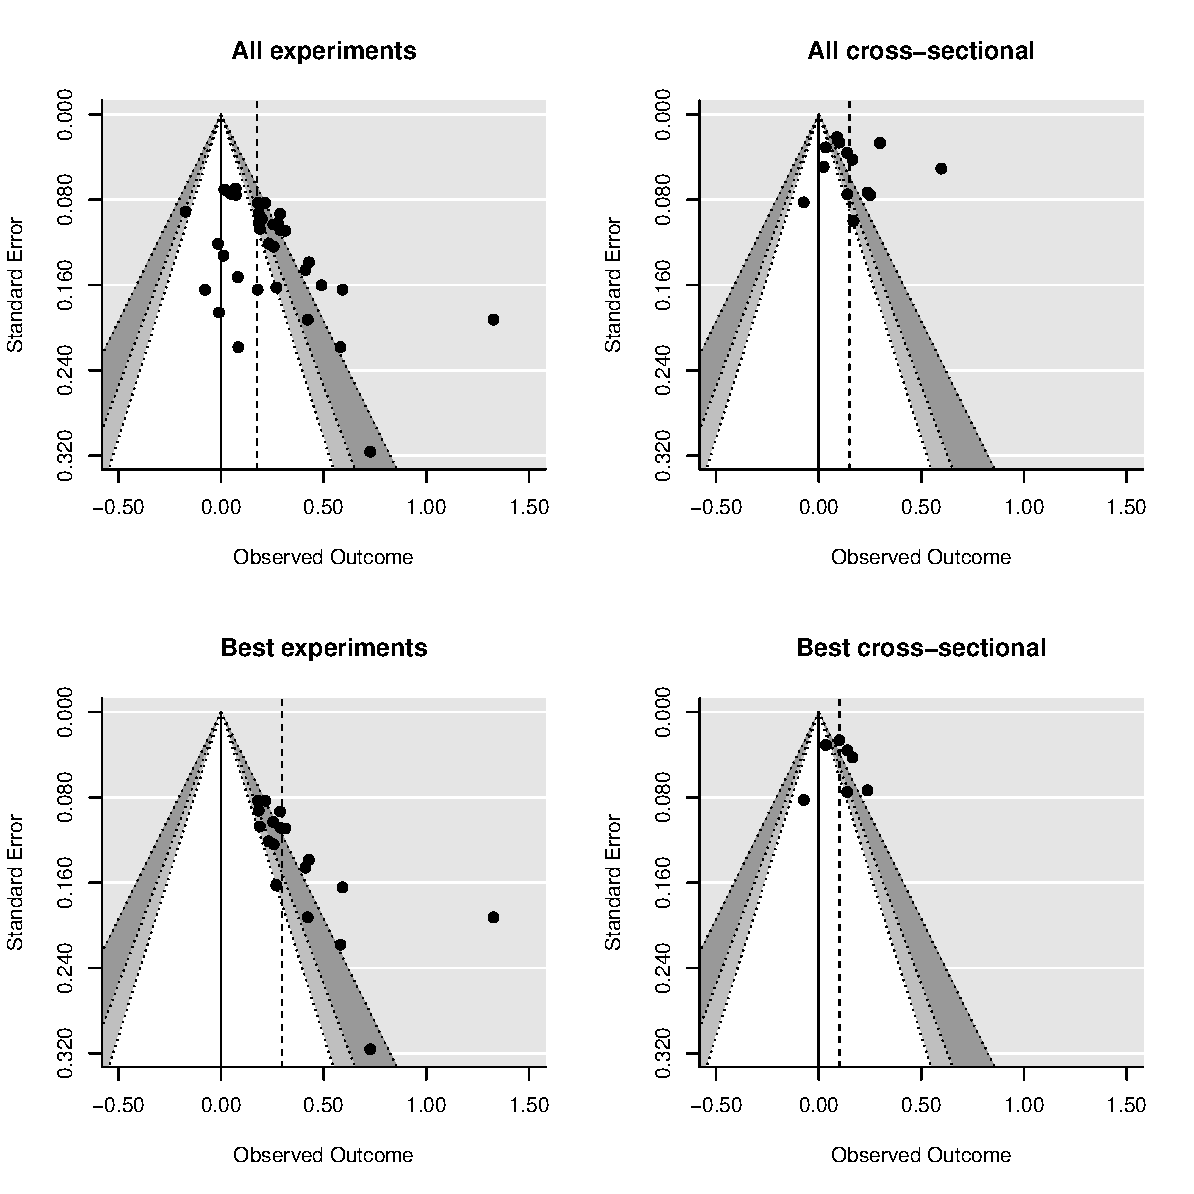
\includegraphics[width = \textwidth, keepaspectratio]{funnels-0_AggAff.pdf}
	\caption{Funnel plot of studies of aggressive affect with overlaid PET and PEESE meta-regression lines. The light and dark shaded regions correspond to two-tailed $p$-values of $p < .10$ and $p < .05$, respectively. The vertical dashed line represents the na{\"i}ve meta-analytic estimate. Application of best-practices criteria seems to emphasize statistical significance, and a knot of experiments just reach statistical significance. One experiment \citep{Ballard:Wiest:1996} finds an implausibly large effect, as does one correlational study.}
	\label{funnel-aggaff}
\end{figure}

\begin{figure}
	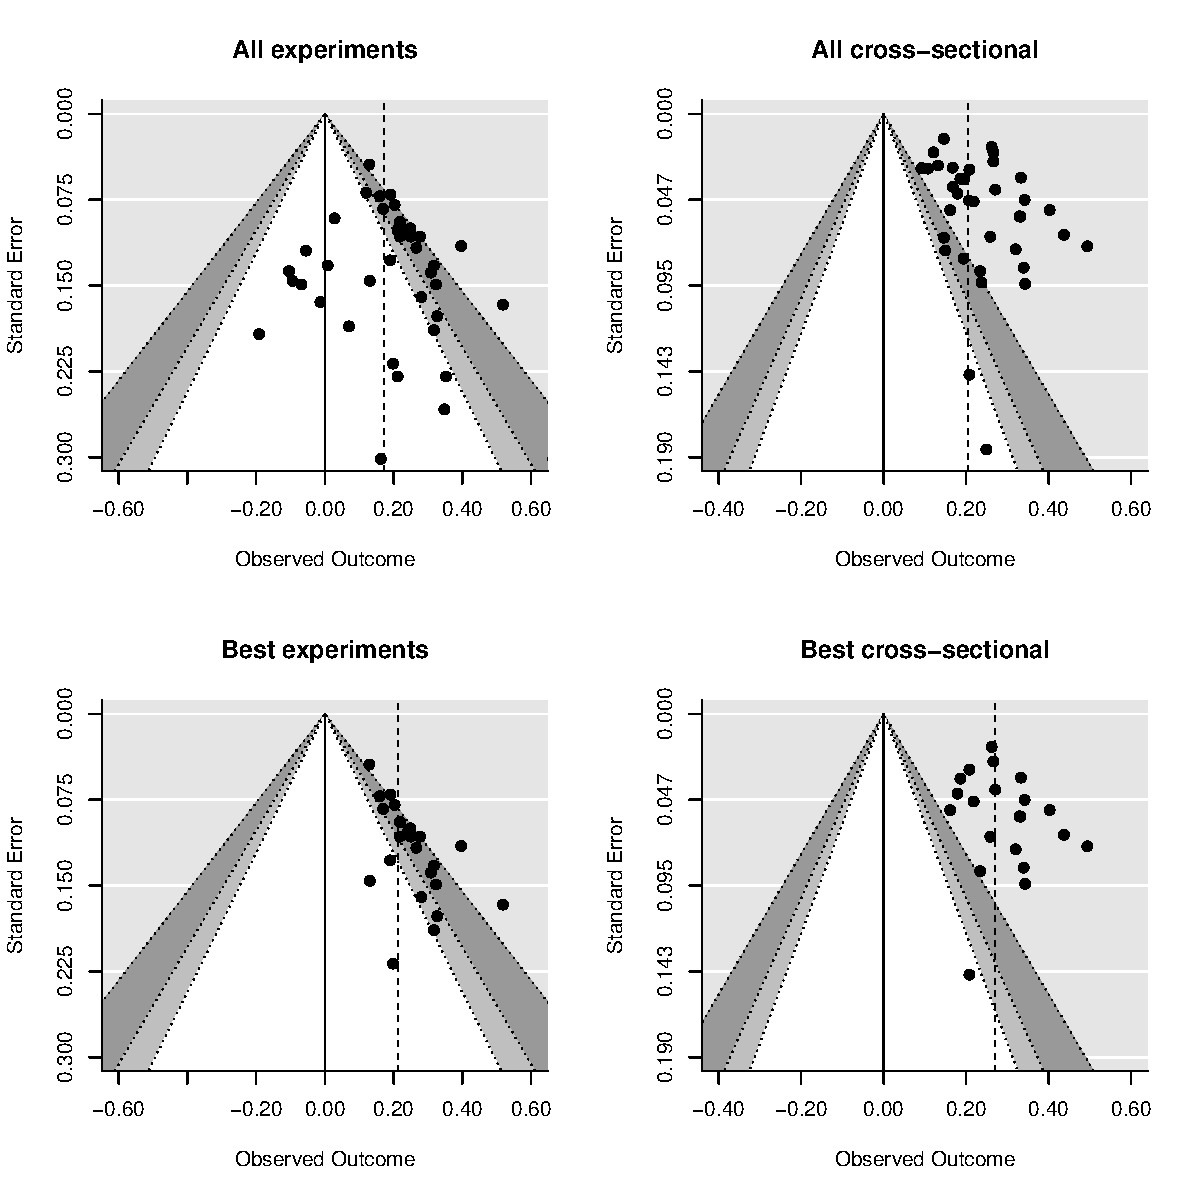
\includegraphics[width = \textwidth, keepaspectratio]{funnels-0_AggBeh.pdf}
	\caption{Funnel plot of studies of aggressive behavior with overlaid PET and PEESE meta-regression lines. The light and dark shaded regions correspond to two-tailed $p$-values of $p < .10$ and $p < .05$, respectively. The vertical dashed line represents the na{\"i}ve meta-analytic estimate. Again, application of best-practices criteria favors experiments finding statistical significance, and studies aggregate in the region $.01 < p < .05$.}
	\label{funnel-aggbeh}
\end{figure}

\begin{figure}
	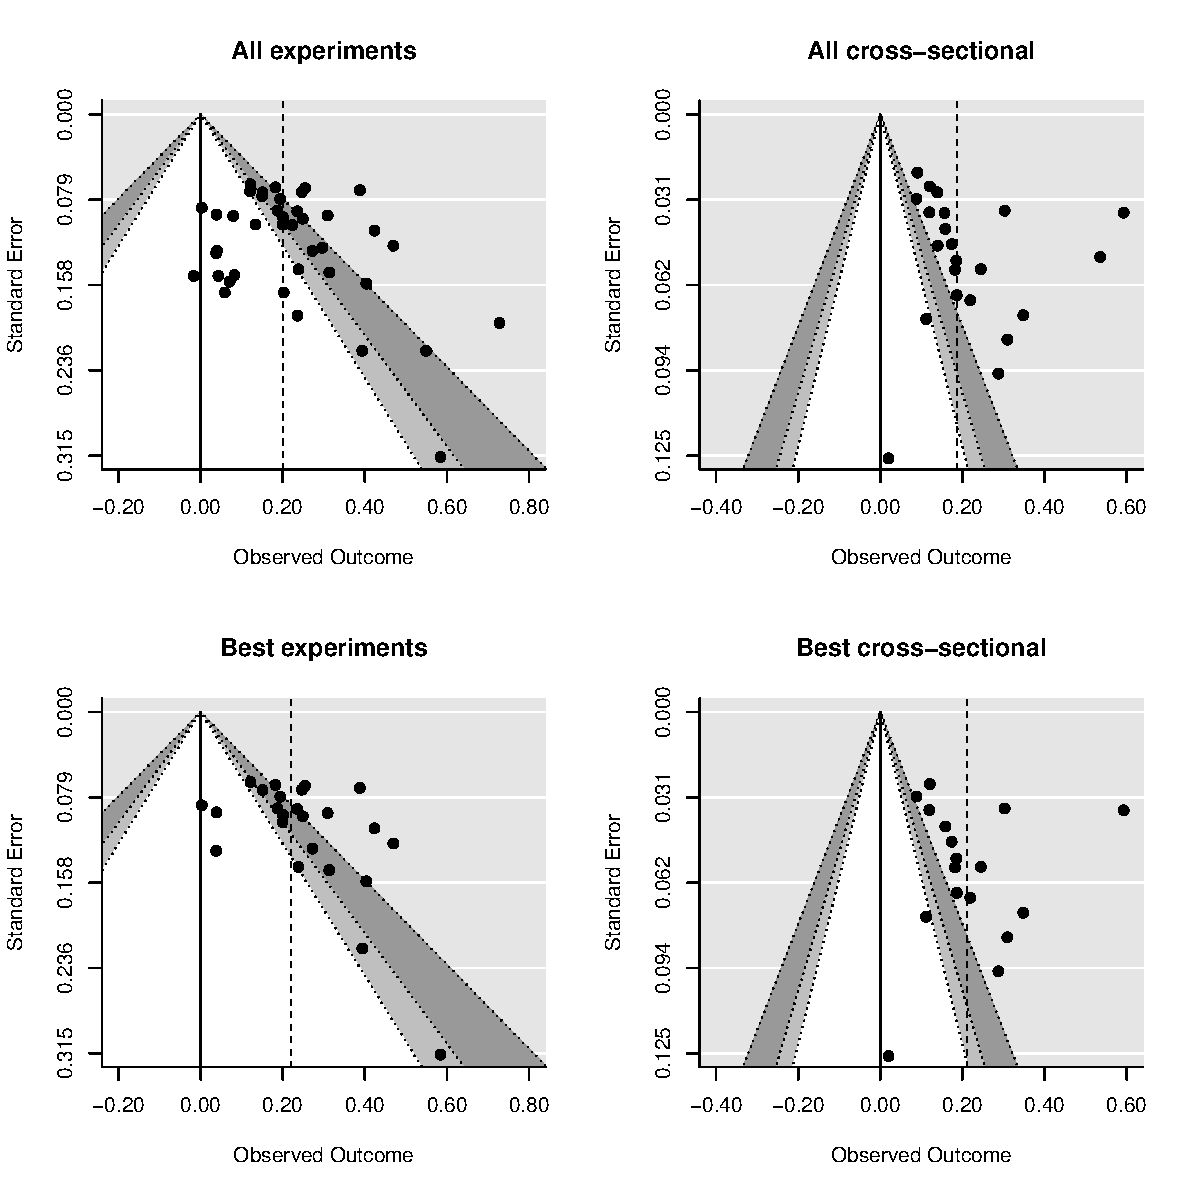
\includegraphics[width = \textwidth, keepaspectratio]{funnels-0_AggCog.pdf}
	\caption{Funnel plot of studies of aggressive cognition with overlaid PET and PEESE meta-regression lines. The light and dark shaded regions correspond to two-tailed $p$-values of $p < .10$ and $p < .05$, respectively. The vertical dashed line represents the na{\"i}ve meta-analytic estimate. Results appear heterogeneous, but less contaminated by bias.}
	\label{funnel-aggcog}
\end{figure}

\begin{figure}
	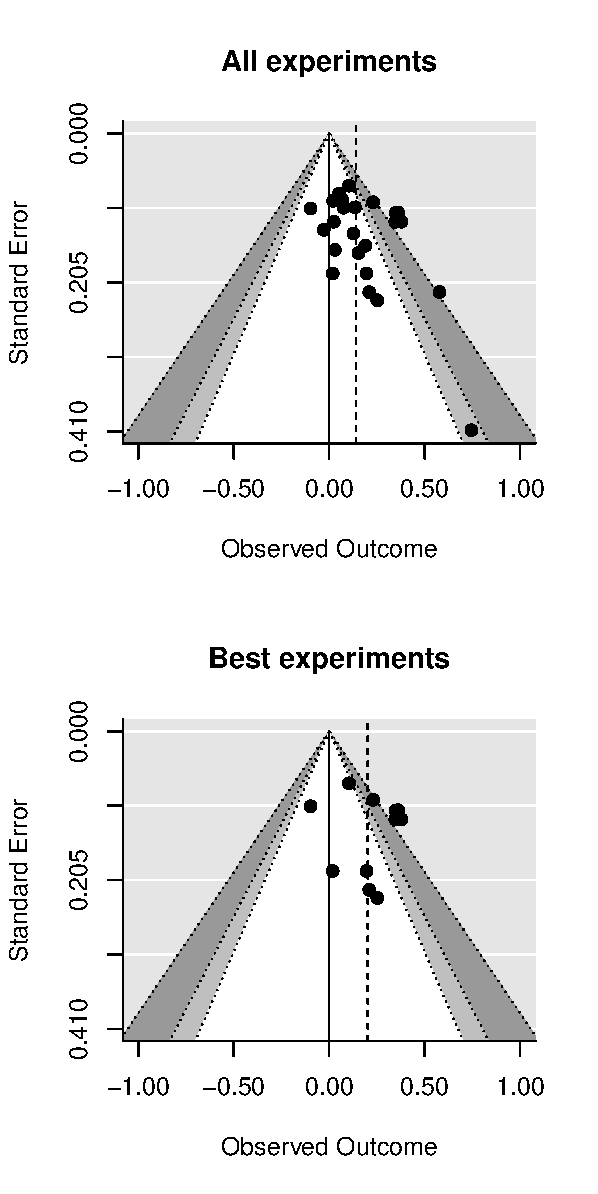
\includegraphics{funnels-0_PhysArous.pdf}
	\caption{Funnel plot of studies of physiological arousal with overlaid PET and PEESE meta-regression lines. The light and dark shaded regions correspond to two-tailed $p$-values of $p < .10$ and $p < .05$, respectively. The vertical dashed line represents the na{\"i}ve meta-analytic estimate. Results do not appear to be systematically contaminated by bias.}
	\label{funnel-physarous}
\end{figure}

\begin{figure}
	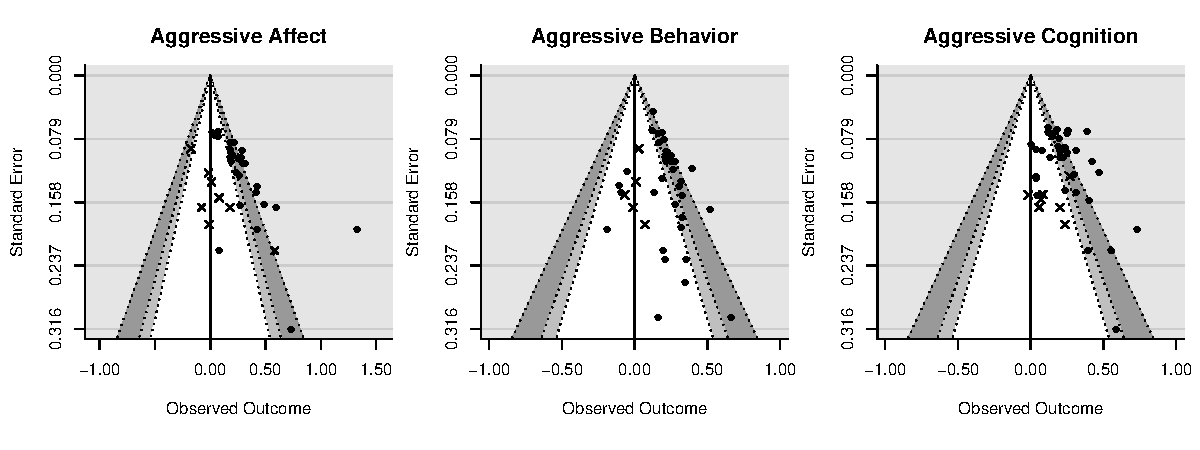
\includegraphics[width = \textwidth, keepaspectratio]{funnel_diss.pdf}
	\caption{Funnel plots of all experiments of aggressive affect, behavior, and cognition. Dissertations not presented in any further publication format are indicated with Xs, while all other publication styles (e.g., journal articles, book chapters, conference proceedings) are indicated with filled dots. Nonsignificant results are less likely to be published, and in the case of experimental studies of affect and of behavior, dissertations suggest substantially smaller effects.}
	\label{funnel-diss}
\end{figure}

% Table generated by Excel2LaTeX from sheet 'adjustment'
\begin{sidewaystable}[htbp]
	\centering
	\caption{PET, PEESE, and $p$-curve adjusted estimates. {\em Note:} K = number of studies; N = total N across studies. $p$ is $p$-value for the significance of the PET estimate. When the PET estimate is significant, it is inferred that the underlying effect is nonzero and PEESE should be favored over PET.}
	\begin{tabular}{rrrrrrrrrrrr}
		\toprule
		&       &       &       &       & \multicolumn{2}{c}{Na{\"i}ve} & \multicolumn{1}{c}{} & \multicolumn{4}{c}{Adjusted} \\
		\midrule
		Outcome & Setting & Sample & K     & N     & \multicolumn{1}{c}{Fixed-effects} & \multicolumn{1}{c}{Random-effects} & \multicolumn{1}{c}{} & \multicolumn{1}{c}{p-curve} & \multicolumn{1}{c}{PET} & \multicolumn{1}{c}{\textit{p}} & \multicolumn{1}{c}{PEESE} \\
		Affect & Experiment & Best  & 18    & 1318  & 0.289 & 0.335 &       & 0.155 & -0.120 & 0.198 & 0.143 \\
		Affect & Experiment & Full  & 34    & 2879  & 0.173 & 0.217 &       & 0.164 & -0.112 & 0.055 & 0.061 \\
		Affect & Cross-Section & Best  & -     & -     & -     & -     &       & -     & -     & -     & - \\
		Affect & Cross-Section & Full  & 14    & 9811  & 0.148 & 0.164 &       & 0.164 & 0.106 & \textbf{< .001} & 0.137 \\
		Behavior & Experiment & Best  & 23    & 2413  & 0.209 & 0.213 &       & 0.071 & 0.072 & 0.188 & 0.150 \\
		Behavior & Experiment & Full  & 39    & 3328  & 0.170 & 0.171 &       & 0.052 & 0.127 & \textbf{0.003} & 0.151 \\
		Behavior & Cross-Section & Best  & 21    & 11615 & 0.263 & 0.277 &       & 0.267 & 0.227 & \textbf{< .001} & 0.253 \\
		Behavior & Cross-Section & Full  & 36    & 28337 & 0.201 & 0.229 &       & 0.226 & 0.152 & \textbf{< .001} & 0.189 \\
		Cognition & Experiment & Best  & 24    & 2887  & 0.217 & 0.222 &       & 0.185 & 0.107 & 0.086 & 0.180 \\
		Cognition & Experiment & Full  & 40    & 4073.5 & 0.210 & 0.216 &       & 0.205 & 0.127 & \textbf{0.008} & 0.164 \\
		Cognition & Cross-Section & Best  & 16    & 7221  & 0.168 & 0.184 &       & 0.172 & 0.099 & \textbf{0.001} & 0.147 \\
		Cognition & Cross-Section & Full  & 21    & 12236 & 0.160 & 0.191 &       & 0.170 & 0.063 & \textbf{0.005} & 0.130 \\
		Arousal & Experiment & Best  & 11    & 833   & 0.199 & 0.210 &       & 0.262 & 0.128 & 0.227 & 0.183 \\
		Arousal & Experiment & Full  & 24    & 1770  & 0.139 & 0.148 &       & 0.269 & -0.005 & 0.942 & 0.085 \\
		\bottomrule
	\end{tabular}%
	\label{table:adjustment}%
\end{sidewaystable}

% Table generated by Excel2LaTeX from sheet 'Egger test'
\begin{table}[htbp]
	\centering
	\caption{Egger's regression test.}
	\begin{tabular}{rrrrrr}
		\toprule
		Outcome & Setting & Sample & \textit{b} & SE(b) & \textit{p} \\
		\midrule
		Affect & Experiment & Best  & 3.667 & 0.780 & \textbf{< .001} \\
		Affect & Experiment & Full  & 2.743 & 0.528 & \textbf{< .001} \\
		Affect & Cross-Section & Best  & -     & -     & \textbf{-} \\
		Affect & Cross-Section & Full  & 1.264 & 0.640 & \textbf{0.048} \\
		Behavior & Experiment & Best  & 1.537 & 0.549 & \textbf{0.005} \\
		Behavior & Experiment & Full  & 0.451 & 0.390 & 0.248 \\
		Behavior & Cross-Section & Best  & 1.117 & 0.483 & \textbf{0.021} \\
		Behavior & Cross-Section & Full  & 1.687 & 0.330 & \textbf{< .001} \\
		Cognition & Experiment & Best  & 1.291 & 0.674 & 0.055 \\
		Cognition & Experiment & Full  & 0.773 & 0.479 & 0.107 \\
		Cognition & Cross-Section & Best  & 1.618 & 0.649 & \textbf{0.013} \\
		Cognition & Cross-Section & Full  & 2.593 & 0.539 & \textbf{< .001} \\
		Arousal & Experiment & Best  & 0.66  & 0.905 & 0.466 \\
		Arousal & Experiment & Full  & 1.292 & 0.626 & \textbf{0.039} \\
		\bottomrule
	\end{tabular}%
	\label{table:Egger}%
\end{table}

% Table generated by Excel2LaTeX from sheet 'dissertation_freqtable'
% Table generated by Excel2LaTeX from sheet 'dissertation_freqtable'
\begin{table}[htbp]
	\centering
	\caption{The statistical significance and best-practices coding of unpublished dissertations.}
	\begin{tabular}{rrrr}
		\toprule
		\multicolumn{3}{c}{\textbf{Liberal coding scheme.}} &  \\
		\midrule
		& \multicolumn{2}{c}{Statistical significance} &  \\
		Publication format & Yes   & No    &  \\
		Other & 168   & 155   &  \\
		Unpublished Dissertation & 3     & 31    &  \\
		&       &       &  \\
		& \multicolumn{2}{c}{Labeled Best Practices} &  \\
		Publication format & Yes   & No    &  \\
		Other & 204   & 119   &  \\
		Unpublished Dissertation & 4     & 30    &  \\
		&       &       &  \\
		\multicolumn{4}{c}{\textbf{Conservative coding scheme.}} \\
		& \multicolumn{3}{c}{Statistical significance} \\
		Publication format & Yes   & Mixed & No \\
		Other & 57    & 42    & 36 \\
		Unpublished Dissertation & 1     & 2     & 16 \\
		&       &       &  \\
		& \multicolumn{2}{c}{Labeled Best Practices} &  \\
		Publication format & Yes   & No    &  \\
		Other & 81    & 63    &  \\
		Unpublished Dissertation & 3     & 16    &  \\
		\bottomrule
	\end{tabular}%
	\label{table:dissertations}%
\end{table}

\end{document}



%Fun quotes
%Donnerstein, Strasburger, Bushman, comparing skepticism to holocaust denial
%Paul Broca proves that women's brains are smaller and that women are inferior
% Gustave Le Bon (1879), ``In the most intelligent races, as among the Parisians, there are a large number of women whose brains are closer in size to those of gorillas than to the most developed male brains. This inferiority is so obvious that no one can contest it for a moment; only its degree is worth discussion. All psychologists who have studied the intelligence of women, as well as poets and novelists, recognize today that they represent the most inferior forms of human evolution and that they are closer to children and savages than to an adult, civilized man.''


%Bushman & Huesmann 2014, p. 51, "Furthermore, the Anderson et al. (2010) meta-analysis included extensive testing for possible publication bias, and found none. [...] In many ways it is quite impressive that playing a violent video game for just 15-30 min, on a single occasion can have significant and measurable effects on aggressive behavior."
%Bushman & Huesmann 2014 cites Carlson, Marcus-Newhall, & Miller 1989 meta-analysis as demonstrating "impressive convergence across a wide range of laboratory aggression measures" and Anderson & Bushman 1997 meta-analysis as finding that "'real' and laboratory measures of aggression are influenced in similar ways by situational variables (e.g., alcohol, provocation, anonymity) and by individual difference variables (e.g., trait aggressiveness, participant sex, Type A personality)."
% Bushman & Huesmann emphasize that Anderson 2010 did not ask -anyone- for -unpublished- studies, and that some unpublished dissertations were found but had been published or had not met the inclusion criteria. [best-practices inclusion criteria??]
% Bushman & Huesmann suggest turning Pearson r into an odds ratio because it sounds more impressive. It is, maybe, if you are willing to assume even odds as priors.
% Parting shot, bagging on Ferguson for writing ``violent prose''.

% Warburton 2014 coming off the top rope talking about "Absolute truths in science are elusive'' but basically arguing that the research attains a reasonable degree of proof.
% "That is, unless there is a credible explanation as to why the effects of violent media (including video games) should be an exception to established findings from other media, or a valid reason why different psychological mechanisms would underlie those effects, it must be assumed that media violence effects are likely to follow patterns similar to those that have already been demonstrated." (maybe they're all bunk because psychologists are knuckleheads)
% Cites Greietemeyer a couple times as part of a ``growing research stream on positive media impacts'' which I aso think are rot based on their terrible power
% Warburton argues that other media does have impact, violence exposure factors have impact, and the processes must be the same as under other social psychological processess. He seems to decide a priori that "violent media can and must have some psychological impact on those who experience it, and probably does so via well-understood psychological processes. Thus, for me, research in media violence no longer needs to establish whether such media can have a psychological and behavioral impact, but should instead rigorously examine the boundary conditions for such impacts." (p 62)
% Warburton claims to have improved the hot sauce paradigm methodologically, Waburton Williams Carins, 2006; Warburton, 2014
% Adorable to see him mis-state p-value. "At law [on the balance of probabilities] is a lesser burden of proof. In science, many effects are tested in this way because statistically, the significance of a finding is usually measured in terms of the probability that it is erroneous (i.e., a Type I error). Most commonly there is a cut-off, a value at which the probability is too high that an effect found is simply due to an error in the study (e.g., a p-value of 5 %). Above the value it is thought that, on the balance of probabilities, an effect is not likely to be real. Below the value, it is thought that, on the balance of probabilities, an effect is likely to be real." Barf!
%Again argues publication bias claim ``strongly refuted'' but Anderson et al., and cite Rothstein & Bushman (2012) as published meta-analysis experts.
% I'm a little bothered by this idea that larger metas are always better. Anderson and Greitemeyer both seem to include a lot of studies and effects I'm not sure really belong in there. They argue selectivity based on their biased best-practices sample but argue massive sample size based on the no-criteria sample.
% See also Bushman, Rothstein, and Anderson about the pub bias argument.
% Warburton talks about the triangulation of experimental, cross-sectional, longitudinal, and brain-imaging research. I see a triangulation of research bias!
% Public policy statement 2000 from AAP, AACAP, APA, AMA, AAFP, APA.

% Barbara Krahe
% Cites Bargh, Chen, Burrows (1996) as definitive evidence of priming effects, lmao. People still believed this stuff in 2014?

% Bushman Rothstein Anderson 2010 Much Ado about Something
% very odd: "The term -unpublished study- means that the study was not published in a peer-reviewed journal, although it could have been published in another outlet (e.g., book)". Chiefly I am concerned about studies that never made it to any public attention (e.g., were swallowed due to $p > .05 %$)
% Cite a bunch of experts as emphasizing searching for books, book chapters, conference proceedings, dissertations, and other "gray" literature. So where is the gray literature?
% This whole article is gold, they harp endlessly upon how important it is that they sought out unpublished studies.
% Talking about "small study effects" but we really know what's going on here.

% For everybody else, everything else has been so consistently statistically significant that they can't fathom this NOT being statistically significant.
% I'm coming from the opposite direction: This is significant or at least exaggerated through dramatic publication and analytic bias. It is hard to believe that the foundational research of the 70s, 80s, 90s that we build upon is similarly biased. If we want to develop a research tool and argue for its efficacy, there are clear right and wrong answers. Research producing the right answer is more likely to be published and accepted than research producing the wrong answer.
% "Spun-glass theory of the mind" -- Meehl, 1973, Why I Do Not Attend Case Conferences